\documentclass[11pt,letterpaper]{article}
\usepackage[margin=0.62in,top=0.69in,bottom=0.66in,headheight=15pt,headsep=13pt,footskip=24pt]{geometry}
\usepackage{tikz,amsmath,amssymb,fancyhdr,array}
\usetikzlibrary{arrows.meta}
\usepackage[T1]{fontenc}\usepackage{lmodern}
\renewcommand{\familydefault}{\sfdefault}
\pagestyle{fancy}\fancyhf{}\fancyhead[L]{\small Week 70 / Shields in a portal room / Grades 4--5}
\fancyfoot[L]{\scriptsize Bellingham Math Circle / Week 70 / GGT70-S-v1}\fancyfoot[R]{\scriptsize\thepage}
\renewcommand{\headrulewidth}{0.4pt}\renewcommand{\footrulewidth}{0pt}
\setlength{\parindent}{0pt}\setlength{\parskip}{8pt}
\newcommand{\problem}[2]{\textbf{Problem #1:} #2\par}

\newcommand{\room}[2]{% scale arrow choice 0 none 1 NE 2 NW 3 SE 4 SW
\begin{tikzpicture}[scale=#1]
\draw[step=1,gray!28,thin] (0,0) grid (4,4);
\draw[thick] (0,0) rectangle (4,4);
\foreach\p in {(0,0),(4,0),(0,4),(4,4)}{\fill\p circle(1.7pt);}
\node[below left,font=\small]at(0,0){S};\node[below right,font=\small]at(4,0){S};
\node[above left,font=\small]at(0,4){S};\node[above right,font=\small]at(4,4){S};
\fill[white](2,2)circle(4pt);\draw[thick](2,2)circle(3pt);\node[above right,font=\small]at(2,2){T};
\node[below,font=\scriptsize]at(2,0){Y};\node[above,font=\scriptsize]at(2,4){Y};
\node[left,font=\scriptsize]at(0,2){X};\node[right,font=\scriptsize]at(4,2){X};
\ifnum#2=1\draw[-{Stealth[length=5pt]},very thick](0,0)--(.65,.65);\fi
\ifnum#2=2\draw[-{Stealth[length=5pt]},very thick](4,0)--(3.35,.65);\fi
\ifnum#2=3\draw[-{Stealth[length=5pt]},very thick](0,4)--(.65,3.35);\fi
\ifnum#2=4\draw[-{Stealth[length=5pt]},very thick](4,4)--(3.35,3.35);\fi
\end{tikzpicture}}
\newcommand{\mapwindow}{
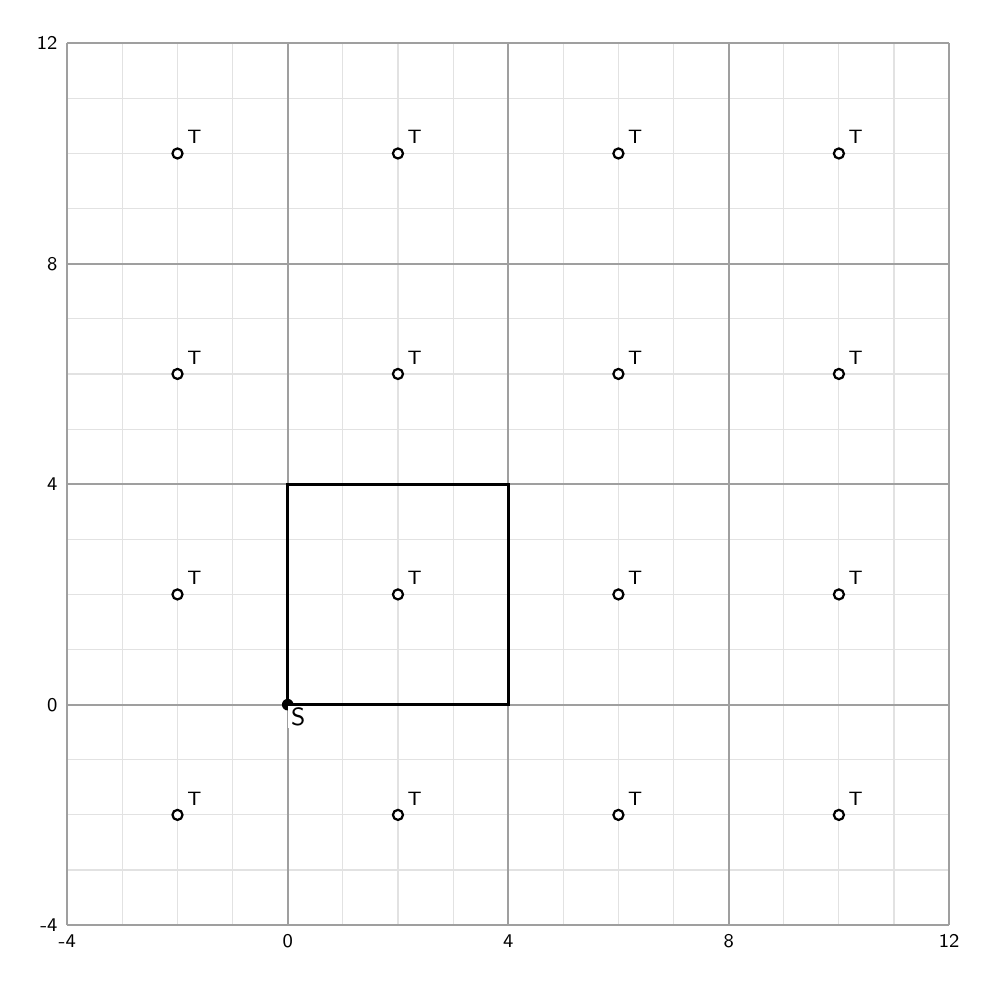
\begin{tikzpicture}[scale=.70]
\draw[step=1,gray!23,thin](-4,-4)grid(12,12);
\foreach\x in{-4,0,4,8,12}{\draw[gray!75,line width=.7pt](\x,-4)--(\x,12);}
\foreach\y in{-4,0,4,8,12}{\draw[gray!75,line width=.7pt](-4,\y)--(12,\y);}
\foreach\x in{-2,2,6,10}{\foreach\y in{-2,2,6,10}{\draw[fill=white,thick](\x,\y)circle(2.6pt);\node[above right,font=\scriptsize]at(\x,\y){T};}}
\fill(0,0)circle(3pt);\node[below right,fill=white,inner sep=1pt,font=\small]at(0,0){S};
\draw[line width=1.2pt](0,0)rectangle(4,4);
\foreach\x in{-4,0,4,8,12}{\node[below,font=\scriptsize]at(\x,-4){\x};}
\foreach\y in{-4,0,4,8,12}{\node[left,font=\scriptsize]at(-4,\y){\y};}
\end{tikzpicture}}
\newcommand{\lines}[1]{\foreach\n in{1,...,#1}{\noindent\rule{\linewidth}{.2pt}\par\vspace{.22in}}}
\begin{document}
A shot travels straight. At an X edge it reappears at the same height on the other X edge. Y edges work the same way, at the same left-to-right position. It keeps its direction. All four corners are the same S. Stop at the first T reached.

A shield is one exact point, away from S and T. A shot stops only if its line passes through that point. A counter marks the point at its center.

\begin{center}
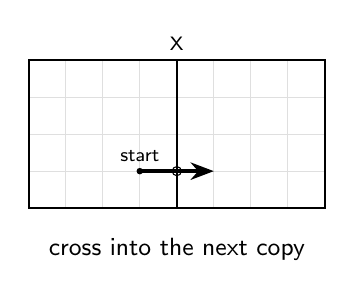
\begin{tikzpicture}[scale=.47]
\draw[step=1,gray!25](0,0)grid(8,4);\draw[thick](0,0)rectangle(4,4);\draw[thick](4,0)rectangle(8,4);
\fill(3,1)circle(2.5pt);\draw[-{Stealth},very thick](3,1)--(5,1);\draw(4,1)circle(3.5pt);
\node[above,font=\scriptsize]at(3,1){start};\node[above,font=\scriptsize]at(4,4){X};
\node[below,font=\small]at(4,-.55){cross into the next copy};
\end{tikzpicture}\hspace{.35in}
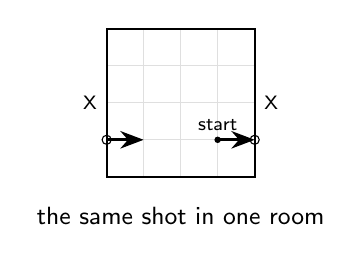
\begin{tikzpicture}[scale=.47]
\draw[step=1,gray!25](0,0)grid(4,4);\draw[thick](0,0)rectangle(4,4);
\fill(3,1)circle(2.5pt);\draw[-{Stealth},very thick](3,1)--(4,1);\draw[-{Stealth},very thick](0,1)--(1,1);
\draw(0,1)circle(3.5pt);\draw(4,1)circle(3.5pt);
\node[above,font=\scriptsize]at(3,1){start};\node[left,font=\scriptsize]at(0,2){X};\node[right,font=\scriptsize]at(4,2){X};
\node[below,font=\small]at(2,-.55){the same shot in one room};
\end{tikzpicture}
\end{center}
\problem{1}{Finish the four diagonal shots. Choose one shield arrangement for the room that stops all four shots. Use as few shields as you can. Your partner checks the shot lines and shields. Swap jobs for a new arrangement.}
\begin{center}
\begin{tabular}{c@{\hspace{.80in}}c}
\room{1.02}{1}&\room{1.02}{2}\\[10pt]
\room{1.02}{3}&\room{1.02}{4}
\end{tabular}
\end{center}
\vfill
Our fewest shields: \rule{.9in}{.3pt}
\newpage
\problem{2}{Choose four different copies of T. Draw a straight shot from S to each. Your partner checks whether a shot passes through an earlier T. In the small room, draw one of your shots as it travels through the portals.}
Each square below is another copy of the same room. Every T is the same target. The bold square is the room shown below the map.
\begin{center}\mapwindow\end{center}
\begin{center}\room{1.05}{0}\end{center}
\newpage
\problem{3}{Find four shield points in the room that stop every shot on the map. Your partner chooses targets and uses straight shots on the map to test your shields. Move your shields until no shot gets through.}
\begin{center}\mapwindow\end{center}
\begin{center}\room{1.05}{0}\end{center}
\newpage
\problem{4}{Find four shield points that stop every straight shot from S to T, even one that goes far beyond the map. Explain why your points work. Could three shields ever stop every shot?}
\vspace{.15in}
\begin{center}\room{1.65}{0}\end{center}
\vspace{.20in}\lines{5}
\end{document}
